\documentclass[conference]{IEEEtran}
\usepackage{amsmath,amssymb,mathtools}
\usepackage{booktabs}
\usepackage{tabularx}
\usepackage{graphicx}
\usepackage{microtype}
\usepackage{tikz}
\usetikzlibrary{arrows.meta,positioning,calc}
\usepackage{xspace}
\usepackage{url}
\graphicspath{{../../generated/}}
% Generated by scripts/make_future_choice_artifacts.py; do not edit.
\newcommand{\FCSharedStaticUnionFalseNeg}{15/15}
\newcommand{\FCDynamicFreshBuildsMax}{192}
\newcommand{\FCDynamicPersistentBuildsMax}{32}
\newcommand{\FCComponentFreshExactC16}{866}
\newcommand{\FCComponentPersistentExactC16}{246}
\newcommand{\FCComponentRecomputesC16}{36}
\newcommand{\FCComponentReusesC16}{62}
\newcommand{\FCNtenCohortSize}{21}
\newcommand{\FCBANNDepthFourZero}{17}
\newcommand{\FCBANNZero}{21}
\newcommand{\FCBANNFallbackPct}{11.3\%}
\newcommand{\FCBANNTotalPct}{25.8\%}
\newcommand{\FCBANNReductionPct}{60.9\%}
\newcommand{\FCGDBDepthFourZero}{20}
\newcommand{\FCGDBZero}{21}
\newcommand{\FCGDBFallbackPct}{16.6\%}
\newcommand{\FCGDBTotalPct}{30.4\%}
\newcommand{\FCGDBReductionPct}{60.3\%}
\newcommand{\FCNDFDepthFourZero}{11}
\newcommand{\FCNDFZero}{21}
\newcommand{\FCNDFFallbackPct}{18.1\%}
\newcommand{\FCNDFTotalPct}{30.9\%}
\newcommand{\FCNDFReductionPct}{60.5\%}
\newcommand{\FCNNDepthFourZero}{17}
\newcommand{\FCNNZero}{21}
\newcommand{\FCNNFallbackPct}{11.3\%}
\newcommand{\FCNNTotalPct}{25.8\%}
\newcommand{\FCNNReductionPct}{60.9\%}

\newcommand{\futurechoice}{\textsc{FutureChoice}\xspace}
\newcommand{\Ob}{\mathcal{O}}
\newcommand{\Worlds}{\mathcal{W}}
\newcommand{\Choices}{\mathcal{F}}
\newcommand{\Res}{\mathcal{R}}
\newcommand{\Evi}{\mathcal{E}}

\title{Preserving Future Choices in Agentic Semantic Communication}
\author{Anonymous Authors}

\begin{document}
\maketitle

\begin{abstract}
Agentic semantic communication increasingly lets an intelligent endpoint decide what to query, transmit, retain, or actuate as task state and communication opportunities evolve. Existing work has made these decisions task-aware through semantic value, goal-oriented state, context relevance, and long-horizon return. We identify a complementary failure mode motivated by pre-disaster emergency monitoring: a communication or information action can be highly useful now yet consume the only energy, contact, or observation-dependent resource needed to satisfy a later hard task requirement. We call the missing object \emph{future-choice feasibility}: whether taking an action preserves at least one non-anticipative policy that can still complete all outstanding hard task semantics under future observations and shared communication opportunities.

We develop \futurechoice, an exact-correct feasibility layer that combines replayable lower certificates, sound optimistic impossibility tests, set-level opportunity-conflict structure, persistent validity domains, and exact fallback. We deliberately separate method hardness from benchmark validity. A source-grounded executable emergency-communication benchmark retains ordinary-solved and negative cases rather than tailoring tasks to the method; an independent public deadline-and-battery mission then tests whether the same abstraction matters outside our simulator. On a frozen 100-instance hard-feasible N=10 cohort, \futurechoice yields zero-tardiness completion for all four released heuristic policies, while depth-4 receding planning leaves residual failures; the first 21 instances are independently audited at 924 reached action frontiers with zero mismatch against exact continuation. Transferring the set-level conflict abstraction from the ASC formulation to a deadline-set MST bound reduces exact-correct search work by roughly 60\% relative to our earlier bound on the frozen exact-audited cohort. These results position future-choice feasibility as a safety/completion complement to semantic value, not as another semantic value metric.
\end{abstract}

\section{Introduction}
Remote pre-disaster monitoring exposes a form of communication difficulty that is easy to miss when an action is judged only by its immediate semantic value. A landslide-monitoring node may have little battery, an uplink may disappear for hours, a gateway may temporarily lose its primary backhaul, and a warning phase may require denser sensing before an operator can restore connectivity. In this setting, a query, fallback transmission, or configuration change does more than reveal or deliver useful information. It also commits future energy, airtime, control opportunities, and queue capacity. An action that is locally legal---and even immediately task-beneficial---can therefore destroy the only remaining way to satisfy a later monitoring obligation.

This problem sits naturally inside Agentic Semantic Communication (ASC). Recent goal-oriented and agentic communication systems decide what and when to acquire or transmit according to task relevance, Grade of Effectiveness, semantic information, context, or long-horizon return~\cite{agheli2025pull,wang2026wmcdt,saz2026logicalsemcom,zhao2026wirelesscontext}. Wireless-agent benchmarks likewise increasingly evaluate semantic/network reasoning and multi-step control~\cite{ferrag2026sixgbench,tong2026wirelessbench,ferrag2026alpha3bench}. These advances answer an increasingly rich version of ``how useful is this communication action for the task?'' They do not, however, explicitly represent whether the action leaves any \emph{causal completion policy} that can still satisfy every outstanding hard task requirement after future observations arrive.

We study this missing feasibility primitive. For a legal history $h_t$ and current action $a$, we define the \emph{future-choice set} $\Choices(h_t,a)$ as the set of non-anticipative continuation policies that can still complete all active hard task obligations for every future observation branch compatible with the policy. The distinction is small but consequential. Consider a hidden state $H\in\{0,1\}$ where querying $H$ now consumes one unit of budget and reveals whether a later task requires $B$ or $C$. One remaining query is sufficient after the observation: query $B$ if $H=0$, otherwise query $C$. A static worst-case reservation that unions both possible future obligations reserves $\{B,C\}$ simultaneously and rejects this valid contingent policy. The error is not an inaccurate semantic value. It is a representation error: mutually exclusive future task semantics were collapsed before the observation that separates them.

\begin{figure*}[t]
\centering
\resizebox{0.98\textwidth}{!}{% Generated by scripts/make_future_choice_figures.py; do not edit.
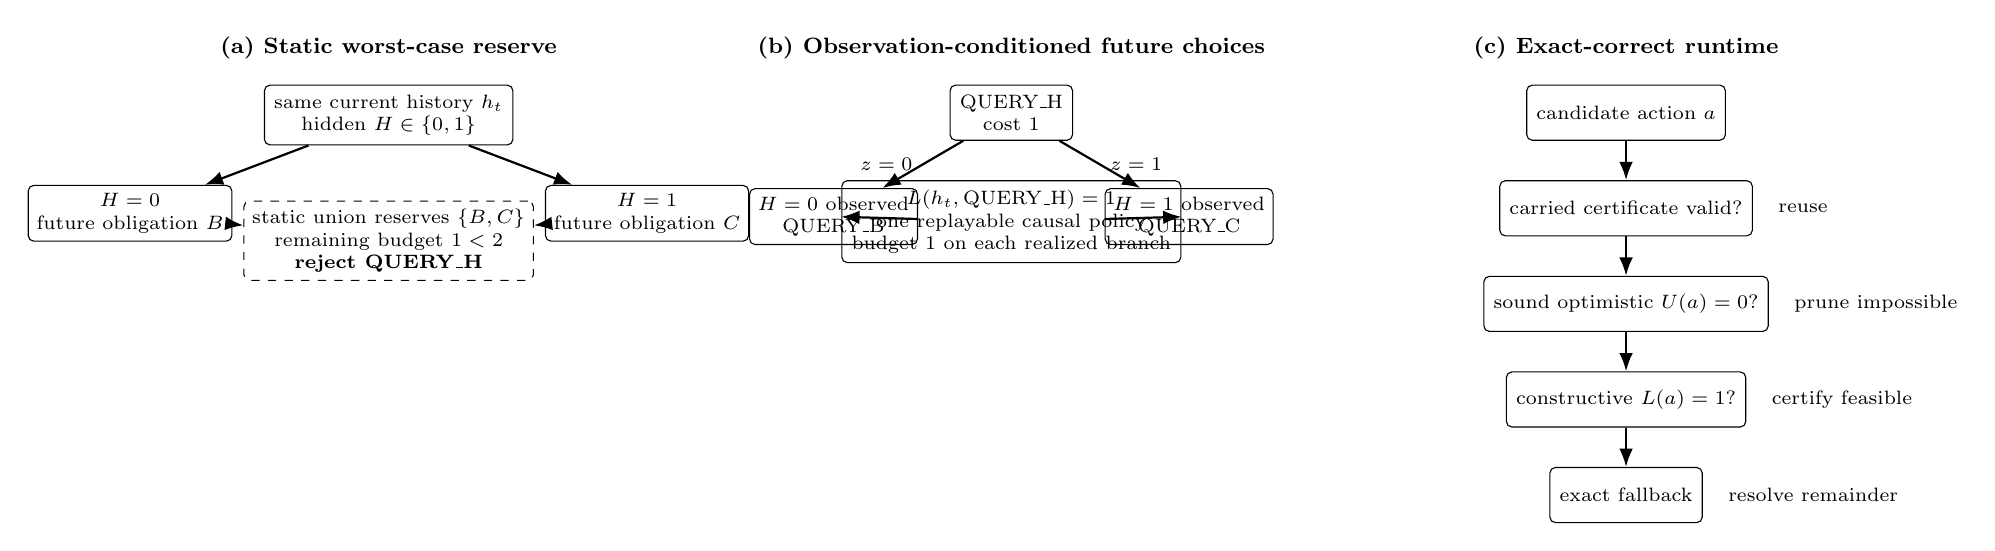
\begin{tikzpicture}[
  >=Latex,
  node distance=5mm and 7mm,
  box/.style={draw, rounded corners=2pt, align=center, inner sep=3.5pt, font=\scriptsize, minimum height=7mm},
  branch/.style={draw, rounded corners=2pt, align=center, inner sep=3pt, font=\scriptsize},
  note/.style={font=\scriptsize, align=center},
  flow/.style={->, line width=.8pt},
  reject/.style={draw, dashed, rounded corners=2pt, align=center, inner sep=3pt, font=\scriptsize},
]
\node[note, font=\footnotesize\bfseries] (ta) {(a) Static worst-case reserve};
\node[box, below=2mm of ta] (h1) {same current history $h_t$\\hidden $H\in\{0,1\}$};
\node[branch, below left=5mm and 4mm of h1] (b) {$H=0$\\future obligation $B$};
\node[branch, below right=5mm and 4mm of h1] (c) {$H=1$\\future obligation $C$};
\draw[flow] (h1) -- (b); \draw[flow] (h1) -- (c);
\node[reject, below=7mm of h1] (union) {static union reserves $\{B,C\}$\\remaining budget $1<2$\\\textbf{reject QUERY\_H}};
\draw[flow, dashed] (b) -- (union); \draw[flow, dashed] (c) -- (union);

\node[note, font=\footnotesize\bfseries, right=23mm of ta] (tb) {(b) Observation-conditioned future choices};
\node[box, below=2mm of tb] (qh) {QUERY\_H\\cost $1$};
\node[branch, below left=6mm and 4mm of qh] (hb) {$H=0$ observed\\QUERY\_B};
\node[branch, below right=6mm and 4mm of qh] (hc) {$H=1$ observed\\QUERY\_C};
\draw[flow] (qh) -- node[note, left] {$z=0$} (hb);
\draw[flow] (qh) -- node[note, right] {$z=1$} (hc);
\node[box, below=5mm of qh] (cert) {$L(h_t,\mathrm{QUERY\_H})=1$\\one replayable causal policy\\budget $1$ on each realized branch};
\draw[flow] (hb) -- (cert); \draw[flow] (hc) -- (cert);

\node[note, font=\footnotesize\bfseries, right=24mm of tb] (tc) {(c) Exact-correct runtime};
\node[box, below=2mm of tc] (a) {candidate action $a$};
\node[box, below=of a] (carry) {carried certificate valid?};
\node[box, below=of carry] (u) {sound optimistic $U(a)=0$?};
\node[box, below=of u] (l) {constructive $L(a)=1$?};
\node[box, below=of l] (ex) {exact fallback};
\draw[flow] (a) -- (carry); \draw[flow] (carry) -- (u); \draw[flow] (u) -- (l); \draw[flow] (l) -- (ex);
\node[note, right=2mm of carry] {reuse};
\node[note, right=2mm of u] {prune impossible};
\node[note, right=2mm of l] {certify feasible};
\node[note, right=2mm of ex] {resolve remainder};
\end{tikzpicture}
}
\caption{Future-choice feasibility complements semantic value. (a) A static worst-case union can reject a valid contingent communication/query policy. (b) Conditioning future obligations on future observations preserves the causal branch structure. (c) \futurechoice keeps exact correctness through carried certificates, sound optimistic pruning, constructive lower certificates, and exact fallback.}
\label{fig:mechanism}
\end{figure*}

Our method is intentionally a feasibility layer rather than a new semantic score. Existing ASC policies may continue to rank actions by semantic value, task utility, or learned return; \futurechoice filters or certifies whether those actions preserve hard completion. It maintains two sound Boolean bounds $L_t(a)\le V^*(h_t,a)\le U_t(a)$. A replayable causal witness gives $L_t(a)=1$; an infeasible optimistic relaxation gives $U_t(a)=0$; only unresolved actions require exact fallback. Set-level obligation--opportunity conflicts are represented with capacity-aware flow certificates, and each certificate carries a validity/dependency domain so that a new history event does not automatically force recomputation.

A central methodological choice is to keep the motivating emergency-communication problem unchanged. We do not add a quota, deadline, or scarce resource after seeing where \futurechoice helps. Instead, we derive an executable benchmark from field/standard requirements and preserve ordinary-solved cases as evidence. This benchmark acts as a \emph{reality authority}: it tells us which task semantics, physical actions, and failure modes are legitimate, while also preventing us from tailoring the environment to the method. In fact, several plausible ``agentic'' mechanisms in the emergency scenario are absorbed by ordinary energy admission, packing, or finite-horizon control. We retain these negative results.

To test whether future-choice feasibility is merely an artifact of our emergency simulator, we use an independent public UAV routing environment with native deadlines, battery, chargers, depot return, finite mission time, and an action mask~\cite{dehghani2026uavattention}. The environment contains locally legal actions that destroy an otherwise feasible zero-tardiness full continuation. On a method-independent 100-instance hard-feasible cohort, \futurechoice removes residual failures left by depth-4 receding planning for all four released heuristic policies; the first 21 instances are an embedded exact-audited cohort with 924 reached action frontiers and zero mismatch. The same set-level conflict idea isolated in ASC further yields a stronger deadline-set MST impossibility bound in the UAV domain, reducing exact-correct search work without changing task outcomes.

We make four contributions:
\begin{itemize}
  \item \textbf{A missing ASC primitive.} We formulate \emph{future-choice feasibility}, separating the semantic value of a current action from whether it preserves any non-anticipative way to complete remaining hard task semantics under future observations and shared opportunities.
  \item \textbf{An exact-correct incremental method.} We develop replayable lower certificates, sound optimistic upper tests, set-level conflict structure, certificate validity domains, and dependency-local invalidation under a common $L/U+$exact-fallback protocol.
  \item \textbf{Reality-grounded evaluation.} We construct a source-grounded executable benchmark for pre-disaster emergency communication and explicitly retain ordinary-solved and negative cases, separating benchmark validity from method hardness.
  \item \textbf{Cross-domain evidence.} We validate the same planning object on an independent deadline-and-battery mission, including an exact-audited correctness cohort, a 100-instance paired scale study, and a direct B$\rightarrow$C attribution in which the ASC set-level conflict abstraction tightens the external domain's sound bound.
\end{itemize}

\section{ASC Problem Setting and Emergency-System Model}
\label{sec:model}
\subsection{From emergency requirements to hard task semantics}
Our primary scenario is pre-disaster mountain monitoring under intermittent communication and limited energy. We retain the system model already used by the source-grounded benchmark rather than introducing a separate planning abstraction. An operational task is
\begin{equation}
\tau=(\mathcal N_\tau,\mathcal M_\tau,\mathcal P_\tau,\mathcal W_\tau,
\mathcal D_\tau,\mathcal A_\tau,\mathcal S_\tau),
\end{equation}
which fixes target nodes and measurands, monitoring profiles, legal windows and deadlines, authorized effects/actions, and a source/scoring profile. A hard task-semantic obligation is
\begin{equation}
o=(i,m,r_o,[s_o,e_o],d_o),
\end{equation}
requiring a valid sample of measurand $m$ from node $i$ in $[s_o,e_o]$ and delivery to the downstream center by $d_o$. This obligation is our executable form of goal-conditioned semantic relevance: it states what information must become available to the downstream task, by when, without prescribing a unique packet trajectory.

The physical communication state includes node batteries and caches, installed sensing/reporting configuration, access/backhaul state, gateway queues, and runtime state. We write
\begin{equation}
x_{t+1}=F(x_t,a_t,\xi_t;\phi),
\end{equation}
where $\xi_t$ contains exogenous harvest, temperature, wireless variation, outages, and task revisions; $\phi$ contains frozen deployment/protocol parameters. The agent does not observe $x_t$ directly. At owner/location $\ell$, legal observations are
\begin{equation}
z_t=H(x_{\le t},a_{<t},\xi_{\le t},\ell),
\end{equation}
and are materialized into an Evidence World $\Evi_t$ that preserves source, owner, generation/observation time, freshness, revision, and status. We use $h_t$ to denote the legal history available to the decision process; hidden simulator truth is excluded.

This maps directly onto goal-oriented ASC: sensing nodes are semantic sources, evidence/query capabilities are semantic acquisition actions, communication/device capabilities are transmission or actuation actions, and the downstream obligation evaluator is the task-effectiveness authority. The key difference from a purely scalar task utility is that some semantics are \emph{hard}: missing their release/window/deadline makes the episode operationally incomplete even if other messages have high semantic value.

\subsection{Why value and feasibility are different}
Let $Q_{\rm sem}(h_t,a)$ be any existing semantic/task-value score. Our objective is not to replace it. We ask whether $a$ is compatible with hard task completion. Let $\Worlds(h_t)$ denote worlds consistent with the legal history, and let $\Ob(w,h)$ be the outstanding hard obligations in world $w$ after history $h$. A continuation policy $\pi$ is \emph{non-anticipative}: two histories exposing the same legal observations must induce the same action until an observation distinguishes them.

We define
\begin{equation}
\begin{aligned}
\Choices(h_t,a)=\{\pi:\ &\forall w\in\Worlds(h_t),\ \forall z\ \text{reachable},\\
&\pi\ \text{legally completes }\Ob(w,h)\},
\end{aligned}
\end{equation}
and the exact feasibility indicator
\begin{equation}
V^*(h_t,a)=\mathbf 1[\Choices(h_t,a)\neq\varnothing].
\end{equation}
A value-driven ASC policy can therefore be wrapped as
\begin{equation}
\max_a Q_{\rm sem}(h_t,a) \quad \text{s.t.}\quad V^*(h_t,a)=1.
\end{equation}
This formulation makes \futurechoice a feasibility/safety complement to semantic value rather than another value metric.

\section{Future-Choice Feasibility}
\label{sec:method}
\subsection{Exact-correct $L/U$ decomposition}
Computing $V^*$ exactly at every decision can be expensive. We maintain Boolean bounds
\begin{equation}
L_t(a)\le V^*(h_t,a)\le U_t(a),\qquad L_t,U_t\in\{0,1\}.
\end{equation}
A replayable causal completion witness sets $L_t(a)=1$. An infeasible \emph{optimistic} relaxation sets $U_t(a)=0$. Actions with $(L,U)=(0,1)$ remain unresolved and fall back to exact search. The runtime order is deliberately conservative: carried certificate reuse, sound $U=0$ pruning, constructive $L=1$ certification, then exact fallback (Fig.~\ref{fig:mechanism}).

\paragraph{Lemma 1 (lower-bound soundness).}
If a certificate provides a legal, non-anticipative continuation that completes every active hard obligation on every compatible observation branch in its validity domain, then $L_t(a)=1$ implies $V^*(h_t,a)=1$.
\emph{Proof sketch.} The replayable certificate is itself an element of $\Choices(h_t,a)$.

\paragraph{Lemma 2 (upper-bound soundness).}
Let $\widetilde P(h_t,a)$ be a relaxation that only removes constraints or adds resources. If $\widetilde P(h_t,a)$ is infeasible, then $U_t(a)=0$ implies $V^*(h_t,a)=0$.
\emph{Proof sketch.} Any real completion would also be feasible in the optimistic relaxation, giving a contradiction.

\subsection{Set-level opportunity conflicts}
Within a compatible branch, we construct a bipartite graph $G=(\Ob,\Res,E)$ between hard obligations and future service opportunities. An edge indicates that a service opportunity can legally complete an obligation. Capacity-aware max-flow gives an optimistic matching; residual min-cuts expose Hall-deficient obligation subsets. The key object is therefore not whether each obligation has \emph{some} candidate opportunity, but whether a set of obligations jointly competes for the same scarce future opportunities.

This representation is observation-conditioned. Future obligations that belong to mutually exclusive observation branches are not statically unioned before the observation arrives. This distinction is what prevents the false-negative reservation pattern in Fig.~\ref{fig:mechanism}.

\subsection{Persistent validity and dependency-local invalidation}
Each certificate stores a validity domain
\begin{equation}
D(c)=(\Worlds_c,[b_{\min},b_{\max}],\mathcal D_c,t_c^{\rm valid},\text{witness}),
\end{equation}
where $\mathcal D_c$ contains the obligations, communication opportunities, and pending execution/evidence events on which the certificate depends. Observation narrowing can shrink $\Worlds_c$ without invalidating the witness. Conversely, a resource or time event invalidates only certificates whose dependency domain changes.

\paragraph{Lemma 3 (dependency-disjoint preservation).}
If an event leaves a certificate's support/resource/time validity domain unchanged, modifies no dependency in $\mathcal D_c$, and introduces no new legal opportunity edge connecting the reused component to another component, the certificate remains valid. If the last condition cannot be guaranteed, the runtime conservatively repartitions or fully rebuilds rather than reusing the certificate.

This lemma captures a systems distinction that ordinary history caches miss: \emph{history changed} does not necessarily imply \emph{future-feasibility structure changed}.

\subsection{A transferable optimistic bound}
The external UAV adapter instantiates the same set-level idea using deadline sets. For each deadline threshold $d$, let $S_d$ be unserved customers due by $d$. Any route prefix serving $S_d$ must form a connected walk spanning the current position and $S_d$, whose length is at least their Euclidean minimum spanning tree. Thus
\begin{equation}
t+\frac{\operatorname{MST}(\{x_t\}\cup S_d)}{v}>d
\quad\Longrightarrow\quad U_t(a)=0.
\end{equation}
Battery limits, charging detours, and depot return are omitted, so the test is optimistic.

\paragraph{Lemma 4 (deadline-set MST soundness).}
If the deadline-set MST inequality above fails for any $d$, no real route can serve all customers in $S_d$ by $d$. Hence pruning the action is sound.

\section{Source-Grounded Emergency Evaluation}
\label{sec:benchmark}
Our benchmark is not constructed around \futurechoice. It is derived independently from field, standard, and procurement requirements for pre-disaster emergency monitoring. This design choice is important: many realistic tasks are in fact saturated by ordinary mechanisms, and we retain them as conformance or interactive-decision cases rather than removing them for lack of method headroom.

The benchmark uses three strata: \emph{Operational-Conformance}, \emph{Interactive-Decision}, and \emph{Future-Choice-Stress}. The first validates source/task/evaluator correctness; the second exercises sequential actions and feedback but may be ordinary-solved; only the third is permitted to support a method-necessity claim. The current paper-facing release contains seven executable T1 surfaces, a frozen 200/200/150 train/dev/test coordinate split, execution-evaluator mutation tests, and a frozen baseline protocol. The 150-coordinate deterministic test produces 750 online baseline rows and 210 bounded oracle diagnostics. A frozen 30-coordinate $\times$ two-context-mode model-spectrum subset is evaluated separately and is not used for the \futurechoice claim.

\begin{figure}[t]
\centering
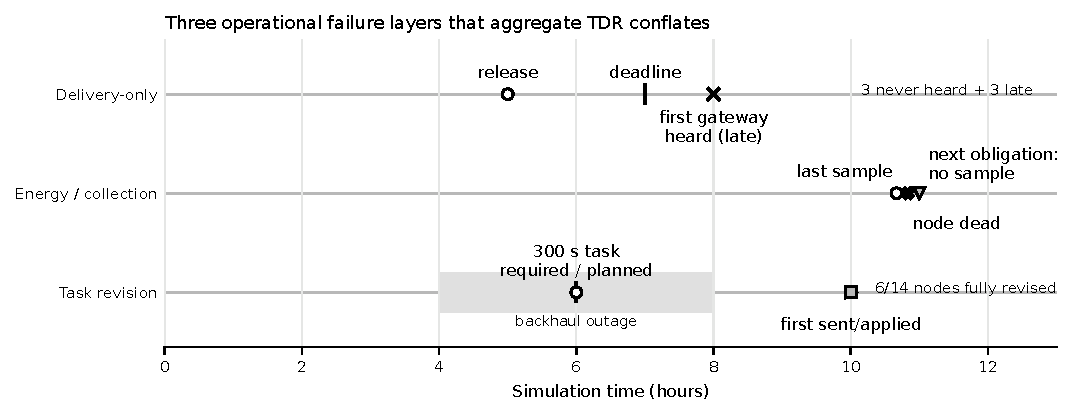
\includegraphics[width=\columnwidth]{fig_layer1_failure_lifecycles.pdf}
\caption{Three rule-selected failure cases from the frozen deterministic test. Delivery-only, energy/collection, and task-revision failures occupy different points in the sensing--gateway--center lifecycle even when an aggregate delivery metric hides the distinction.}
\label{fig:failures}
\end{figure}

Figure~\ref{fig:failures} illustrates why final-state/lifecycle evaluation matters. In the delivery-only case, sensing succeeds but some samples never reach the gateway and others arrive after the deadline. In the energy case, the node dies before the next required sample exists. In the task-revision case, the denser task becomes active during a backhaul outage and only a subset of nodes installs both required settings. These are different operational failures and should not be collapsed into one ``bad communication'' score.

\section{Evaluation Methodology}
\label{sec:evaluation}
We organize evaluation around five research questions rather than around code modules.

\begin{table*}[t]
\centering
\caption{Frozen experiment design. Scale experiments and correctness experiments are deliberately separated: large panels extend statistical stability, while exact-frontier audits remain on bounded preregistered cohorts.}
\label{tab:design}
\footnotesize
% Generated by scripts/make_future_choice_artifacts.py; do not edit.
\begin{tabularx}{\textwidth}{@{}lXX@{}}
\toprule
RQ & Evidence family and frozen scale & Correctness / control gate\\
\midrule
RQ1 & Emergency benchmark validity. 150 frozen coordinates; 750 online rows; 210 oracle diagnostics & source/evaluator audit + frozen deterministic test\\
RQ2 & Conditional ASC representation. 20 exact-audited cells; 18 cells; 15 nontrivial & exact contingent feasibility vs static union/reserve\\
RQ3 & Incremental correctness / structure. C=2,4,8,16; 4 unseen B6 graph motifs & fresh rebuild + persistent/dependency exact controls\\
RQ4 & External mission outcomes. 21 constructive seeds x 4 policies; 924 exact frontier checks; 100 of 126 constructive seeds from scan 0..999; first 21 exactly equal C2 exact-audited cohort & 924 exact frontiers + paired depth-4 / scale statistics\\
RQ5 & Cross-domain transfer. Same exact-audited N=10 cohort + generic engine parity & set-MST attribution + shared L/U orchestration\\
\bottomrule
\end{tabularx}

\end{table*}

\textbf{RQ1: Is the emergency benchmark valid, and are realistic tasks all hard?} We audit source-to-task provenance, execution-evaluator mutations, ordinary deterministic baselines, and lifecycle failures. Negative/saturated cases are retained.

\textbf{RQ2: When do scalar value and static reservation fail?} Controlled ASC families isolate observation-conditioned obligations and shared opportunity conflicts, comparing value/static-union views with exact contingent feasibility.

\textbf{RQ3: Can the structure be maintained exactly and incrementally?} We compare fresh exact, ordinary persistent exact, dependency-cache exact, and incremental conflict certificates; a separately frozen structural holdout changes graph motifs rather than merely increasing size.

\textbf{RQ4: Does preserving future choices change outcomes outside our benchmark?} We use the public deadline/battery UAV environment. The main exact-correct cohort has 21 method-independent constructive hard-feasible seeds and 924 independently checked frontiers. A confirmatory scale panel extends to 100 constructive hard-feasible seeds, while a separate 50-episode panel exactly matches the external repository's published evaluation seed protocol.

\textbf{RQ5: Do the ASC and UAV results instantiate the same abstraction?} We attribute the external-domain search reduction to the set-level conflict bound and route both domains through the same generic \futurechoice orchestration protocol.

All exact or large-scale experiments follow a resource-safe execution contract; timeout or memory limits are reported as unresolved computation, never as infeasibility. We report task quality and search/recomputation work separately and do not translate heterogeneous internal work units into wall-clock speedup claims.

\section{Results}
\label{sec:results}
\subsection{RQ1: Reality first---many emergency tasks are ordinary-solved}
The benchmark study finds that several plausible ``agentic'' mechanisms are absorbed by ordinary controls: persistent-energy commitment can be handled by horizon-aware resource admission; shared backup stress can be absorbed by packing/max-coverage rules; and source-valid warning handoff tasks do not justify inventing an unobserved cross-stage contact quota. These negative results support the benchmark's role as a method falsifier rather than a method generator.

\subsection{RQ2--RQ3: Conditional structure is necessary and maintainable}
Static union reservation produces false negatives whenever future obligations belong to mutually exclusive observation branches. The shared-opportunity stress family preserves a local per-branch backup requirement while the static union grows with the number of branches. Persistent conditional domains avoid rebuilding inactive branch frontiers, and active-branch events invalidate only dependency-intersecting components.

We additionally froze a structural holdout \emph{before} execution, replacing the development pattern of equal disconnected components with four unseen graph motifs: asymmetric components, a bridged pair, a chain that splits as shared opportunities disappear, and mixed local/global invalidation. Across all four motifs and every frozen event, the incremental structural snapshot is canonically identical to a fresh full rebuild. The holdout also exposes the intended safety boundary: bridge removal expands or splits the affected dependency scope, while a global satellite-budget change invalidates all backup-dependent components. Under a separate 512~MiB/30~s exact-control budget, six events are resolved by fresh, ordinary persistent, and dependency-cache exact; all six yield identical action frontiers. The remaining exact cells are reported only as unresolved computation.

The mixed local/global motif also uncovered an implementation bottleneck in our optimistic physical upper test: combined terrestrial/satellite assignment was implemented by exponential DFS although the constraint is an integral max-flow with a shared satellite-budget pool. Replacing the DFS with an exhaustively cross-checked max-flow leaves all prior non-timing results unchanged and makes the structural holdout tractable. We treat this as an implementation correction, not as a planner-level wall-clock superiority claim.

\begin{table}[t]
\centering
\caption{ASC representation and maintenance evidence. Work units are intentionally reported without converting component recomputations into exact-search expansions.}
\label{tab:asc}
\resizebox{\columnwidth}{!}{% Generated; do not edit.
\begin{tabular}{lll}
\toprule
Mechanism & Result & Unit / boundary\\
\midrule
Static union & 15/15 false negatives & representation failure\\
Observation narrowing & 192 to 32 builds & persistent domains\\
Fresh ordered exact & 866 & exact expansions\\
Persistent exact & 246 & exact expansions\\
Dependency-cache exact & 246 & separator replay=0\\
Conflict frontier & 36 recompute / 62 reuse & different work unit\\
\bottomrule
\end{tabular}
}
\end{table}

\begin{figure}[t]
\centering
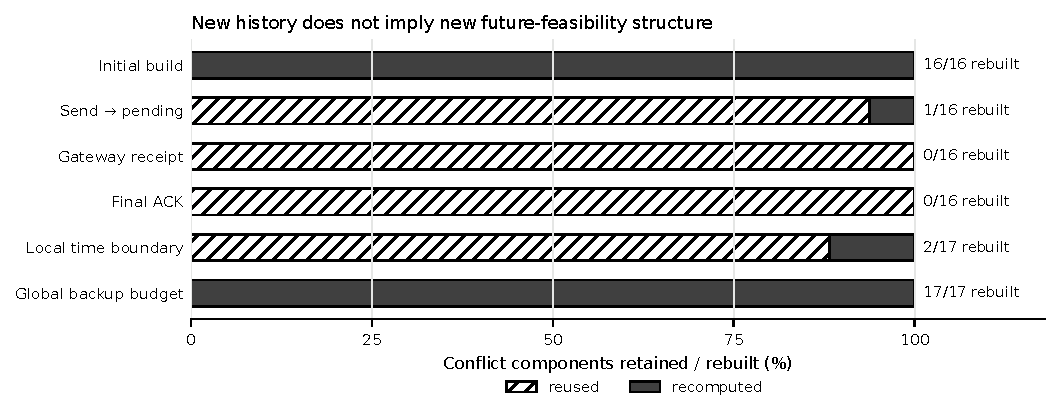
\includegraphics[width=\columnwidth]{fig_dependency_local_invalidation.pdf}
\caption{Dependency-local invalidation for a 16-component revealed branch. A new gateway receipt or final ACK changes history but requires no conflict-component rebuild once the accepted send already secures the obligation; a global backup-budget change invalidates all dependent components.}
\label{fig:invalidation}
\end{figure}

\subsection{RQ4: External task-quality headroom beyond depth-4}
On the frozen 100-instance hard-feasible N=10 cohort, \futurechoice obtains zero-tardiness completion on all four released heuristic policies. Depth-4 receding planning still leaves residual failures, especially for the nearest-deadline policy. Importantly, the first 21 instances are exactly the previously frozen exact-audited cohort; thus correctness and scale are nested rather than being established on unrelated samples.

\begin{figure}[t]
\centering
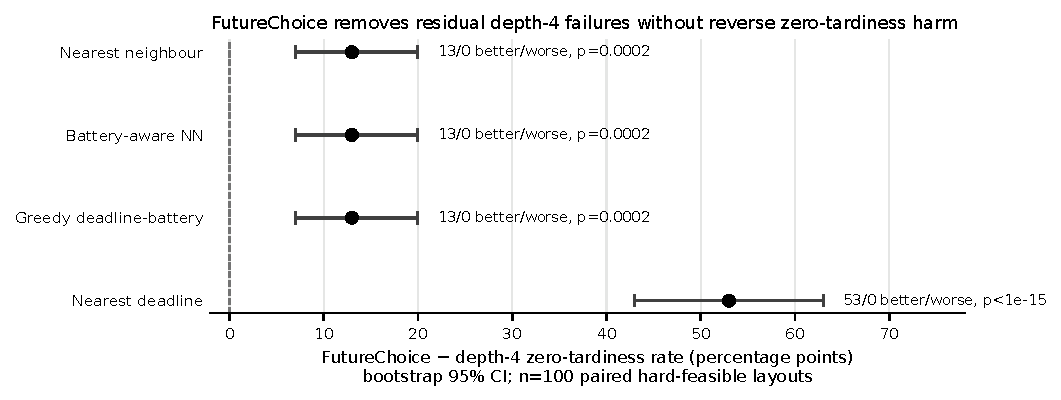
\includegraphics[width=\columnwidth]{fig_uav_paired_gain.pdf}
\caption{Paired zero-tardiness gain of \futurechoice over depth-4 receding planning on 100 preselected hard-feasible N=10 layouts. Error bars are paired bootstrap 95\% confidence intervals; annotations show favorable/adverse discordance and exact McNemar tests.}
\label{fig:pairedgain}
\end{figure}

\begin{table}[t]
\centering
\caption{N=10 scale-confirmatory outcomes on 100 method-independent hard-feasible layouts. The first 21 are the exact-audited cohort.}
\label{tab:scale}
\resizebox{\columnwidth}{!}{% Generated; do not edit.
\begin{tabular}{lrrrrrrr}
\toprule
Policy & Native zero & Depth-4 zero & Future zero & Depth-4 comp. & Future comp. & Depth-4 infeas. & Future infeas.\\
\midrule
Nearest neighbour & 49/100 & 87/100 & 100/100 & 100/100 & 100/100 & 0 & 0\\
Nearest deadline & 12/100 & 47/100 & 100/100 & 69/100 & 100/100 & 41 & 0\\
Greedy deadline-battery & 79/100 & 87/100 & 100/100 & 98/100 & 100/100 & 3 & 0\\
Battery-aware NN & 49/100 & 87/100 & 100/100 & 100/100 & 100/100 & 0 & 0\\
\bottomrule
\end{tabular}
}
\end{table}

\subsection{RQ5: The set-level abstraction transfers}
Replacing an individual-deadline/global-MST optimistic bound with the ASC-inspired deadline-set conflict bound leaves task outcomes unchanged while reducing exact fallback and total exact-correct search work on the frozen exact-audited cohort.

\begin{figure}[t]
\centering
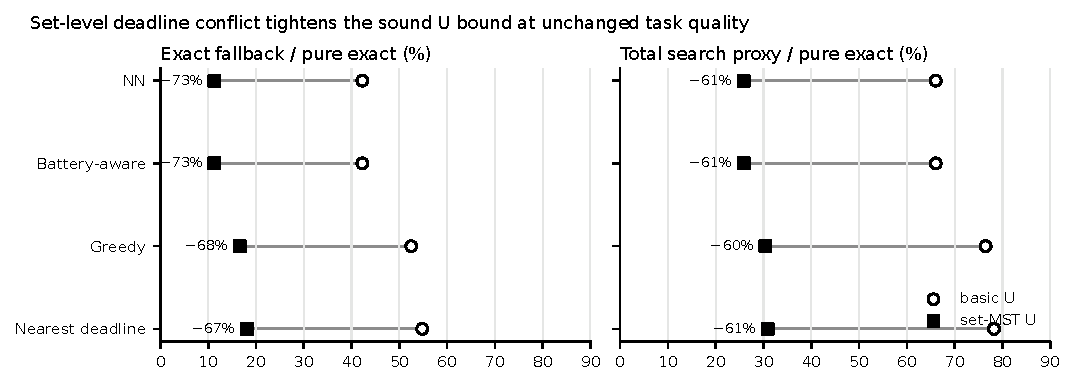
\includegraphics[width=\columnwidth]{fig_setmst_ablation.pdf}
\caption{B$\rightarrow$C attribution. The deadline-set MST bound reduces exact fallback and total exact-correct search work relative to the earlier basic optimistic bound at unchanged task quality.}
\label{fig:setmst}
\end{figure}

The resulting correctness--compute picture is deliberately not a universal dominance claim. Within exact-correct methods, the set-level bound dominates the older basic bound and pure exact-mask point under the declared search-state proxy. Once depth-4 is included, depth-4 and \futurechoice are both non-dominated: depth-4 is cheaper but leaves residual hard-feasibility failures, whereas \futurechoice buys exact-correct completion at higher search cost.

\section{Related Work}
\label{sec:related}
\paragraph{Semantic and goal-oriented communication.}
Semantic communication has progressively moved from representation efficiency toward task effectiveness and goal-oriented decision making~\cite{uysal2021semantic,guo2025semcomnet}. Pull-based scheduling explicitly optimizes what and when to query under long-term semantic effectiveness and query cost~\cite{agheli2025pull}; logical goal-oriented communication builds decision-relevant semantic states~\cite{saz2026logicalsemcom}; world-model semantic communication estimates long-horizon counterfactual contribution to physical-AI return~\cite{wang2026wmcdt}; and wireless context engineering treats context selection and injection as a wireless resource-allocation problem~\cite{zhao2026wirelesscontext}. \futurechoice complements these scalar or representational objectives with a hard completion-feasibility layer.

\paragraph{Agentic wireless systems and benchmarks.}
Recent work brings foundation models and agents into wireless control, tool use, and network management~\cite{liang2025llmwireless,lu2026wirelessops}. 6G-Bench and WirelessBench provide broad semantic/network reasoning benchmarks, while $\alpha^3$-Bench evaluates safety, robustness, and efficiency for UAV agents~\cite{ferrag2026sixgbench,tong2026wirelessbench,ferrag2026alpha3bench}. DORA provides expert-authored operational disaster tasks and replayable tool trajectories~\cite{dora2026}. Our benchmark instead traces emergency-communication requirements into executable communication lifecycles and final hard-obligation outcomes; its role in this paper is to ground and falsify the method rather than to make every task algorithmically hard.

\paragraph{Active information acquisition and constrained planning.}
Decision-region determination, action-sufficient representations, stochastic Boolean evaluation, and adaptive probing all study how much information is needed for a decision~\cite{javdani2014drd,huang2022asr,deshpande2013sbfe,hellerstein2022adaptivity}. Active measuring further models delayed negative effects of measurement itself~\cite{gao2026activemeasuring}. Our distinction is that the controlled communication action changes a set of future hard obligations/opportunities under future observations; we maintain executable completion certificates and their validity domains rather than only a measurement value or stopping criterion.

\section{Discussion and Limitations}
Our current implementation establishes exact action-feasibility and structured work reduction, not universal wall-clock superiority. Ordinary persistent exact search remains a strong systems baseline, and depth-4 receding planning is a cheaper operating point on some external policies. The emergency benchmark's Future-Choice-Stress stratum may remain empty: method evidence comes from the direct ASC formulation and independent external mission rather than from retrofitting scarcity into the benchmark. The N=15 routing result is a bounded probe, not a distribution-level result. The source/task/evaluator audit is internal rather than independent domain-expert validation. The frozen LLM benchmark subset uses one provider/model family and remains a model-spectrum diagnostic, not a contribution to the \futurechoice method claim.

\section{Conclusion}
Agentic semantic communication should not be defined by adding an LLM or another semantic-value score. The difficult regime arises when current communication and information actions change which future hard task completions remain possible. \futurechoice makes this regime explicit through observation-conditioned completion sets, replayable feasibility certificates, sound optimistic impossibility tests, and dependency-local maintenance. A source-grounded emergency benchmark keeps the method tied to legitimate operational semantics, while an independent deadline-and-battery mission shows that the same planning object matters outside the motivating simulator. Our results support future-choice feasibility as a complementary safety layer around existing ASC value policies.

\bibliographystyle{IEEEtran}
\bibliography{../../refs}
\end{document}
